\documentclass{article}
\usepackage{mathrsfs}
\usepackage{harpoon}
\usepackage{comment}
%\usepackage{ctex}
\usepackage{color}
\usepackage{amsmath}
\usepackage{mathtools}
\usepackage{simplewick} 
\usepackage{graphicx} % added for subfig
\usepackage{subfigure} % added for subfig
\usepackage{listings} % added for code block
\title{Note for 2pt calculation with Chroma}
\author{Jinchen He}
\date{}
\usepackage[a4paper,left=20mm,right=20mm,top=20mm,bottom=20mm]{geometry}
\begin{document}
\maketitle
%\tableofcontents
%\pagebreak[4]
\section{Chroma Installation}

\subsection{Download package}

Download necessary packages for Installation from GitHub.

\begin{itemize}
    \item Use "git clone --recursive \dots", "recursive" means after the clone is created, initialize all submodules within, using their default settings.
    \item If the connection to the GitHub is not stable on the server, you are suggested to clone on your local machine, then use "scp" to upload.
\end{itemize}

Package list:

\begin{enumerate}
    \item qmp
    \item qio
    \item qla
    \item qdp
    \item qopqdp
    \item qdpxx
\end{enumerate}

\subsection{Configure and make}

Configure and make in each folder of packages.

\begin{itemize}
    \item The whole process can be divided into 7 parts (6 packages above and chroma), so that you can locate the errors conveniently.
    \item "export PATH=\dots:\$PATH", makes environment variables available to other programs called from bash. 
    \item "autoreconf -vi": used to update generated configuration files, "-v" means verbosely reporting processing, "-i" means copying missing auxiliary files.
    \item "./configure", you can use "./configure –help" to see the options
    \item "./autogen.sh"
\end{itemize}

\section{Source code}

\subsection{Plug in packages}

Users are allowed to write some plug in packages and register in the Chroma, so that those packages can be used.

\subsection{Make}

\begin{itemize}
    \item Makefile
    \item make.sh 
\end{itemize}

\section{2pt calculation}

\subsection{Perl script}

Used to print the .xml file as the input for Chroma.

Write perl script as the structure in "xxx.h".

\subsubsection{Sink smear}

\begin{lstlisting}[language=Python]
    print <<"EOF";
    <elem>
      <Name>SINK_SMEAR</Name>
      <Frequency>1</Frequency>
      <Param>
        <version>5</version>
        <Sink>
          <version>1</version>
          <SinkType>POINT_SINK</SinkType>
          <j_decay>3</j_decay>
        </Sink>
      </Param>
      <NamedObject>
        <gauge_id>$gauge_id</gauge_id>
        <prop_id>${prop_sum}</prop_id> 
        <smeared_prop_id>prop_m${quark_mass}_p${quark_mom_x}${quark_mom_y}
        ${quark_mom_z}.sum_sp</smeared_prop_id>
      </NamedObject>
    </elem>
    EOF
\end{lstlisting}

This block read the propagator in $<prop\_id> </prop\_id>$, then use the method in $<SinkType> </SinkType>$, and output the smeared propagator as $<smeared\_prop\_id> </smeared\_prop\_id>$.


\subsection{Inline xxx.cc}



\subsection{Inline xxx.h}
In perl script,

\begin{lstlisting}[language=Python]
    <s1_quark_props>
    <elem>prop_m${c_mass}_p000.sum_sp</elem>
  </s1_quark_props>
\end{lstlisting}

So, in the $inline\_xxx.h$,

\begin{lstlisting}[language=Python]
    multi1d<std::string> s1_quark_props; 
\end{lstlisting}

here just need to read the name of the variable, which is a string, because the $Sink smear$ block in perl script told Chroma to output a smeared propagator with name $xxx.sum\_up$, and here we just need to let Chroma know which variable should be used.

\subsection{Add new plug in packages}

If you want to use a new plug in package in the Chroma for calculation, you should:

\begin{enumerate}
    \item Write the .cc file and .h file.
    \item Put two files above into the source code folder.
    \item In the source code folder, add '\#include "inline\_xxx.h" ' and "foo \&= InlinexxxEnv::registerAll();" into "chroma.cc".
    \item In the source code folder, add "inline\_2pt.h" and "inline\_2pt.o" into "Makefile".
    \item "bash make.sh" again
    \item Update your .pl file to use the new plug in package, and remake the soft link of "chroma" in the same path as .pl file.
    \item "sbatch xxx.sh" again.
\end{enumerate}


\subsection{Change to use different configurations}

If you want to use other different configurations:

\begin{enumerate}
  \item In the perl script, change "cfg file" and "cfg type", which are configuration path and configuration type.
  \item In the perl script, change "ns" and "nt", which are numbers of lattice on space axes and time axis.
  \item In the perl script, change "mg layout".
  \item In the perl script, change $<tseq>xx</tseq>$ in the EOF block.
\end{enumerate}

\begin{figure}[h]
  \centering
  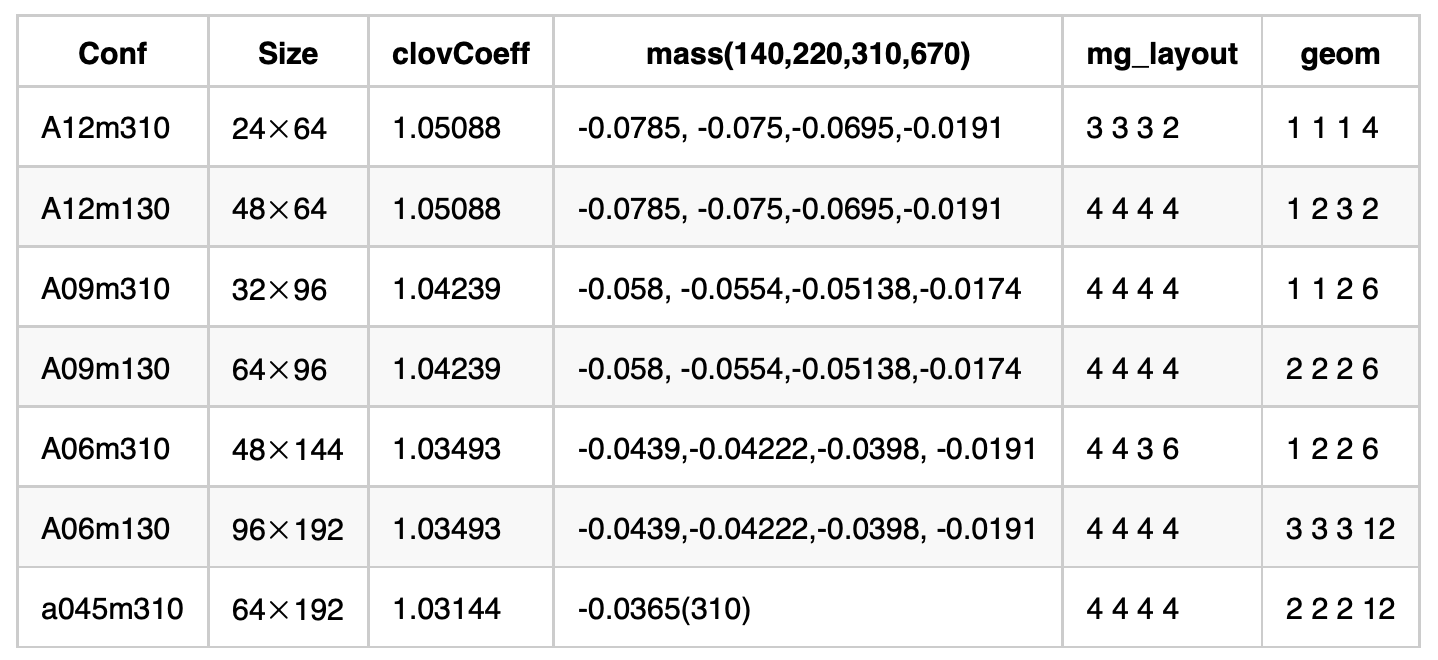
\includegraphics[scale=0.5]{configuration_set.png} 	
\end{figure} 


\end{document}